In section \ref{subsec:general_design} we present an overview of the implementation. Afterwards, we divide the functionalities in 3 parts; in section \ref{subsec:training} we present the methods used for training (fitting) the model, in section \ref{subsec:inference} those used for performing the inference and in section \ref{subsec:evaluation} those used for evaluating the approximate posterior and the obtained samples. 

\subsubsection{General design} 
\label{subsec:general_design}
In figure \ref{fig:romc_overview} we present an overview of our
implementation; one may interpret figure~\ref{fig:romc_overview} as a
depiction of the main class of our implementation, called
\pinline{ROMC}, while the entities inside the green and blue
ellipses are the main functions of the class. Following Python's
naming principles, the methods starting with an underscore (green
ellipses) represent internal (private) functions and are not meant to
be used by a user, whereas the rest of the methods (blue ellipses) are
the functionalities the user interacts with. As mentioned before, the
implementation favours extensibility; the building blocks that compose
the method have been designed in a modular fashion so that a
practitioner may replace them without the method to collapse.

Figure \ref{fig:romc_overview} groups the ROMC implementation into the
training, the inference and the evaluation part. The training part includes all the
steps until the computation of the proposal regions; sampling the
nuisance variables, defining the optimisation problems, solving them,
constructing the regions and fitting local surrogate models. The
inference part comprises of evaluating the unnormalised posterior (and
the normalised one, in low-dimensional cases), sampling and computing
an expectation. Moreover, the ROMC implementation provides some
utilities for inspecting the training process, such as plotting the
histogram of the distances
$d^*_i = g_i(\theta_i^*), \: \forall i \in \{1, \ldots, n_1 \}$ after
solving the optimisation problems and visualising the constructed
bounding box\footnote{if the parametric space is up to $2D$}. Finally,
two functionalities for evaluating the inference are implemented; (a)
computing the Effective Sample Size (ESS) of the weighted samples and
(b) measuring the divergence between the approximate posterior the
ground-truth, if the latter is available.\footnote{Normally, the
  ground-truth posterior is not available; However, this functionality
  is useful in cases where the posterior can be computed numerically
  or with an alternative method (i.e.\ ABC Rejection Sampling) and we
  would like to measure the discrepancy between the two
  approximations.}
  
\subsubsection*{Parallelising the processes}

As stated above, the most critical advantage of the ROMC method is that it can be fully parallelised. In our implementation, we have exploited this fact by implementing a parallel version in the following tasks; (a) solving the optimisation problems, (b) constructing bounding box regions, (c) sampling and (d) evaluating the posterior. Parallelism has been achieved using the package \pinline{multiprocessing}. The specific package enables concurrency, using subprocesses instead of threads, hence side-stepping the Global Interpreter (GIL). In our implementation we use the \pinline{Pool} object, which offers a convenient means of parallelising the execution of a function across multiple input values (data parallelism). For activating the parallel version of the algorithms, the user has to just pass the argument \pinline{parallelize=True} at the initialisation of the \pinline{ROMC} method.


\subsubsection*{Simple one-dimensional example}

For illustrating the functionalities we choose as running example the
following model, introduced by~\autocite{Ikonomov2019},

\begin{gather} \label{eq:1D_example} p(\theta) =
\mathcal{U}(\theta;-2.5,2.5)\\ p(y|\theta) = \left\{
    \begin{array}{ll} \theta^4 + u & \mbox{if } \theta \in [-0.5, 0.5]
\\ |\theta| - c + u & \mbox{otherwise}
    \end{array} \right.\\ u \sim \mathcal{N}(0,1)
\end{gather}

\noindent

In the model \eqref{eq:1D_example}, the prior is the uniform
distribution in the range $[-2.5, 2.5]$ and the likelihood a Gaussian
distribution. There is only one observation $y_0 = 0$. The inference
in this particular example can be performed quite easily, without
incorporating a likelihood-free inference approach. We can exploit this
fact for validating the accuracy of our implementation. The
ground-truth posterior, approximated computationally, is shown in
figure \ref{fig:example_gt}.

\begin{figure}[h]
    \begin{center}
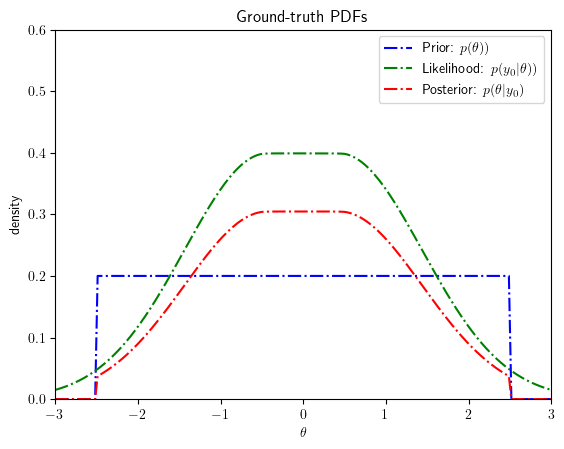
\includegraphics[width=0.7\textwidth]{./Thesis/images/chapter3/example_gt.png}
    \end{center}
  \caption[Ground-truth posterior distribution of the simple 1D
example.]{Ground-truth posterior distribution of the simple 1D
example.}
  \label{fig:example_gt}
\end{figure}

\subsubsection*{ELFI code for modelling the example}

In the following code snippet, we code the model at \textit{ELFI} and
we initialise the ROMC inference method. We observe that the
initialisation of the ROMC inference method is quite intuitive; we
just pass the final (distance) node of the simulator as argument, as
in all $\textit{ELFI}$ inference methods. The argument
\pinline{bounds}, although optional, is important for many
functionalities (e.g. approximating the partition function, setting
the bounds of the Bayesian optimisation etc.) so it is recommended to
be passed.

\begin{pythoncode}
  import elfi import scipy.stats as ss
  import numpy as np
  
  def simulator(t1, batch_size=1,random_state=None):
      if t1 < -0.5:
          y = ss.norm(loc=-t1-c, scale=1).rvs(random_state=random_state)
      elif t1 <= 0.5:
          y = ss.norm(loc=t1**4, scale=1).rvs(random_state=random_state)
      else:
          y = ss.norm(loc=t1-c, scale=1).rvs(random_state=random_state)
      return y

  # observation
  y = 0
      
  # Elfi graph
  t1 = elfi.Prior('uniform', -2.5, 5)
  sim = elfi.Simulator(simulator, t1, observed=y)
  d = elfi.Distance('euclidean', sim)

  # Initialise the ROMC inference method
  bounds = [(-2.5, 2.5)] # limits of the prior
  parallelize = True # activate parallel execution
  romc = elfi.ROMC(d, bounds=bounds, parallelize=parallelize)
\end{pythoncode}


\begin{figure}[!ht]
    \begin{center}
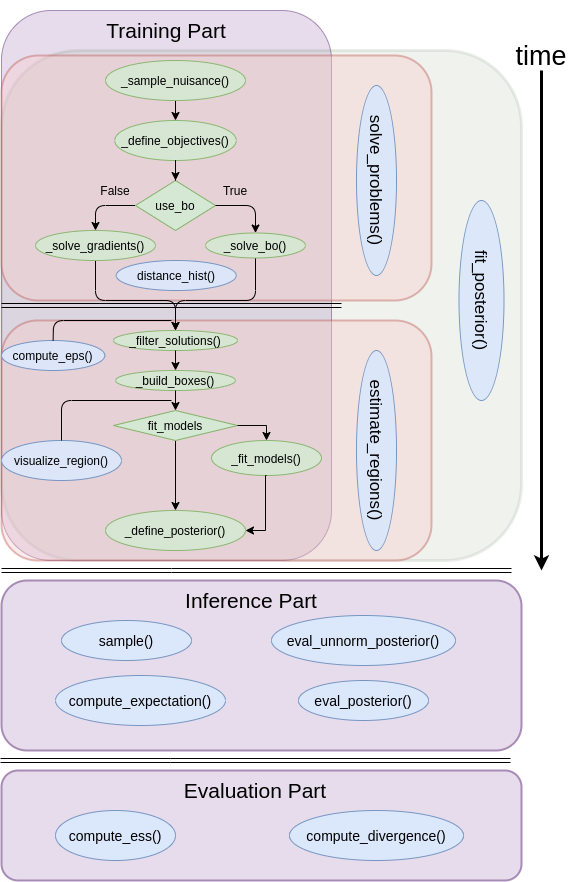
\includegraphics[width=0.8\textwidth]{./Thesis/graphs/ROMC.png}
    \end{center}
    \caption[Overview of the ROMC implementation.]{Overview of the
ROMC implementation. The training part follows a sequential pattern;
the functions in the green ellipses must be called in a sequential
fashion for completing the training part and define the posterior
distribution. The functions in blue ellipses are the functionalities
provided to the user.}
    \label{fig:romc_overview}
\end{figure}

  

\subsubsection{Training part} 
\label{subsec:training}
The training part contains the following 6 functionalities:

\begin{enumerate}[label=(\roman*)]
\item \mintinline{python}{romc.solve_problems(n1, use_bo=False, optimizer_args=None, seed=None)}
\item \mintinline{python}{romc.estimate_regions(eps_filter,}
  
      \mintinline{python}{                      use_surrogate=None, region_args=None,}
  
      \mintinline{python}{                      fit_models=False, fit_models_args=None,}
  
      \mintinline{python}{                      eps_region=None, eps_cutoff=None)}
      
    \item \mintinline{python}{romc.fit_posterior(n1, eps_filter, use_bo=False, optimizer_args=None,}
  
          \mintinline{python}{                   seed=None, use_surrogate=None, region_args=None,}
  
          \mintinline{python}{                   fit_models=False, fit_models_args=None,}
  
          \mintinline{python}{                   eps_region=None, eps_cutoff=None)}

\item \mintinline{python}{romc.distance_hist(savefig=False, **kwargs)}
\item \mintinline{python}{romc.visualize_region(i, savefig=False)}
\item \mintinline{python}{romc.compute_eps(quantile)}
\end{enumerate}


\subsubsection*{Function (i): Define and solve the optimisation problems}

\pinline{romc.solve_problems(n1, use_bo=False, optimizer_args=None, seed=None)}
\vspace{5mm}

\noindent
This routine is responsible for (a) drawing the nuisance variables,
(b) defining the optimisation problems and (c) solving them using either a
gradient-based optimiser or Bayesian optimisation. The aforementioned
tasks are done in a sequential fashion, as show in
figure~\ref{fig:romc_overview}. The definition of the optimisation
problems is performed by drawing $n_1$ integer numbers from a discrete
uniform distribution $u_i \sim \mathcal{U}\{1, 2^{32}-1\}$. Each
integer $u_i$ is the seed used in ELFI's random simulator. Hence from
an algorithmic point-of-view drawing the state of all random
variables $\vb_i$ as described in the previous chapter, traces back to
just setting the seed that initialises the state of the pseudo-random
generator, before asking a sample from the simulator.

Finally, passing an integer number as the argument \pinline{seed}
absorbs all the randomness of the optimisation part (e.g.\ drawing
initial points for the optimisation procedure), making the whole
process reproducible and deterministic.

Setting the argument \pinline{use_bo=True}, chooses the Bayesian
Optimisation scheme for obtaining $\thetab_i^*$. In this case, apart
from obtaining the optimal points $\thetab_i^*$, we also fit a Gaussian
Process (GP) as surrogate model $\hat{d}_i$. In the following steps,
$\hat{d}_i(\thetab)$ will replace $g_i(\thetab)$ when calling the
indicator function.

\subsubsection*{Function (ii): Construct bounding boxes and fit local surrogate models}

\mintinline{python}{romc.estimate_regions(eps_filter,}
  
      \mintinline{python}{                      use_surrogate=None, region_args=None,}
  
      \mintinline{python}{                      fit_models=False, fit_models_args=None,}
  
      \mintinline{python}{                      eps_region=None, eps_cutoff=None)}
\vspace{5mm}

This routine constructs the bounding boxes around the optimal points
$\thetab_i^* : i = 1, 2, \ldots, n_1$ following
Algorithm~\ref{alg:region_construction}. The Hessian matrix is
approximated based on the Jacobian $\hess_i = \jac_i^T \jac_i$. The
eigenvectores are computed using the function
\pinline{numpy.linalg.eig()} that calls, under the hood, the
\pinline{_geev LAPACK}. A check is performed so that the matrix
$\hess_i$ is not singular; if this is the case, the eigenvectors are
set to be the vectors of the standard Euclidean basis i.e.\
$\{ \mathbf{e_1} = (1, 0, \ldots), \mathbf{e_2} = (0,1,0,\ldots),
\text{etc} \}$. Afterwards, the limits are obtained by repeteadly querying
the distance function ($g_i(\thetab)$ or $\hat{d}(\thetab)$) along the
search directions. In section \ref{subsec:developers}, we provide some
details regarding the way the bounding box is defined as a class and
sampling is performed on it.

\subsubsection*{Function (iii): Perform all training steps in a single call}

\mintinline{python}{romc.fit_posterior(n1, eps_filter, use_bo=False, optimizer_args=None,}
  
          \mintinline{python}{                seed=None, use_surrogate=None, region_args=None,}
  
          \mintinline{python}{                fit_models=False, fit_models_args=None,}
  
          \mintinline{python}{                eps_region=None, eps_cutoff=None)}

\vspace{5mm}
\noindent

This function merges all steps for constructing the bounding box into
a single command. If the user doesn't want to manually inspect the
histogram of the distances before deciding where to set the threshold
$\epsilon$, he may call \pinline{romc.fit_posterior()} and the whole
training part will be done end-to-end. There are two alternatives for
setting the threshold $\epsilon$; the first is to set to a specific
value blindly and the second is to set at as a specific quantile of
the histogram of distances. In the second scenario the
\pinline{quantile} argument must be set to a floating number in the
range $[0,1]$ and \pinline{eps='auto'}.


\subsubsection*{Function (iv): Plot the histogramm of the optimal points}

\pinline{romc.distance_hist(**kwargs)}
\vspace{5mm}
\noindent


This function can serve as an intermediate step of manual inspection,
for helping the user choose which threshold $\epsilon$ to use. It
plots a histogram of the distances at the optimal point
$g_i(\thetab_i^*) : \{i = 1, 2, \ldots, n_1\}$ or
$d_i^*$ in case \pinline{use_bo=True}. The function accepts all
keyword arguments and forwards them to the underlying
\pinline{matplotlib.hist()} function; in this way the user may
customise some properties of the histogram, such as the number of bins
or the range of values.

\subsubsection*{Function (v): Plot the acceptance region of the objective functions}

\pinline{romc.visualize_region(i)}
\vspace{5mm}
\noindent

It can be used as an inspection utility for cases where the parametric
space is up to two dimensional. The argument $\pinline{i}$ is the
index of the corresponding optimization problem i.e.\ $i<n_1$.

\subsubsection*{Function (vi): Compute $\epsilon$ automatically based on the distribution of $d^*$}

\pinline{romc.compute_eps(quantile)}
\vspace{5mm}
\noindent

\noindent
This function return the appropriate distance value $d_{i=\kappa}^*$
where $\kappa = \lfloor \frac{quantile}{n} \rfloor$ from the
collection $\{ d_i^* \} \forall i = \{1, \ldots, n\}$ where $n$ is the
number of accepted solutions. It can be used to automate the selection
of the threshold $\epsilon$, e.g.\
\pinline{eps=romc.compute_eps(quantile=0.9)}.


\subsubsection*{Example}

Here we will illustrate the aforementioned functionalities using the
simple 1D example we set up in the previous section. The following
code snippet performs the training part in ELFI.

\begin{pythoncode}
  n1 = 500 # number of optimisation problems
  seed = 21 # seed for solving the optimisation problems
  eps = .75 # threshold for bounding box
  use_bo = False # set to True for switching to Bayesian optimisation

  # Training step-by-step
  romc.solve_problems(n1=n1, seed=seed, use_bo=use_bo)
  romc.theta_hist(bins=100)
  romc.estimate_regions(eps=eps)
  romc.visualize_region(i=1)

  # Equivalent one-line command
  # romc.fit_posterior(n1=n1, eps=eps, use_bo=use_bo, seed=seed)
\end{pythoncode}

As stated before, switching to the Bayesian optimisation scheme needs
nothing more the setting the argument \pinline{use_bo=True}; all the
following command remain unchanged. In figure
\ref{fig:example_training_hist} we illustrate the distribution of the
distances obtained and the acceptance area of the first optimisation
problem. We observe that most optimal points produce almost zero
distance.

\begin{figure}[h]
    \begin{center}
      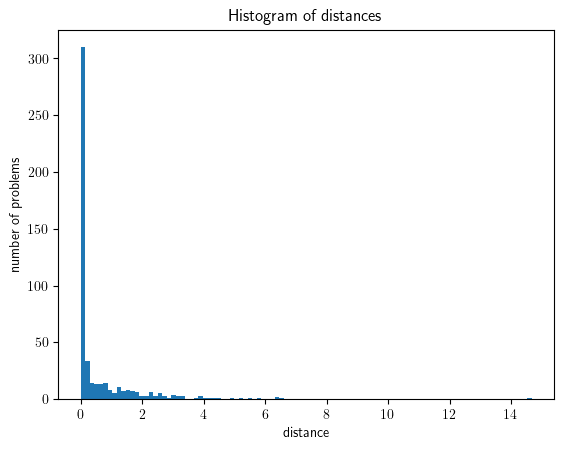
\includegraphics[width=0.48\textwidth]{./Thesis/images/chapter3/example_theta_dist.png}
      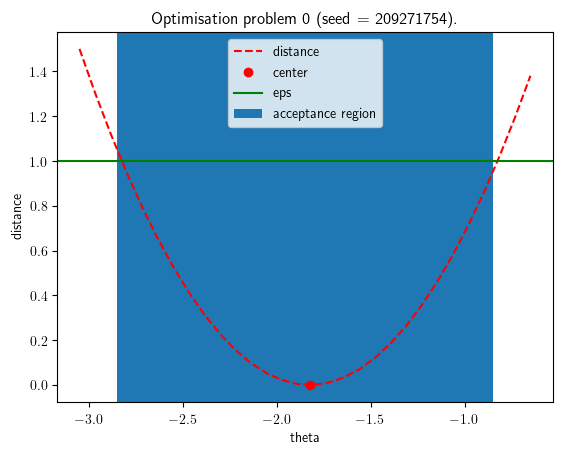
\includegraphics[width=0.48\textwidth]{./Thesis/images/chapter3/example_region.png}
    \end{center}
  \caption[Histogram of distances at the 1D example.]{Histogram of distances and visualisation of a specific region.}
  \label{fig:example_training_hist}
\end{figure}


\subsubsection{Inference part} 
\label{subsec:inference}
The inference part contains the 4 following functionalities:

\begin{enumerate}[label=(\roman*)]
\item \mintinline{python}{romc.sample(n2, seed=None)}
\item \mintinline{python}{romc.compute_expectation(h)}  
\item \mintinline{python}{romc.eval_unnorm_posterior(theta)}
\item \mintinline{python}{romc.eval_posterior(theta)}
\end{enumerate}

\subsubsection*{Function (i): Perform weighted sampling}

\mintinline{python}{romc.sample(n2)}
\vspace{5mm}

\noindent
This is the basic inference utility of the ROMC implementation; we
draw $n_2$ samples for each bounding box region. This gives a total of
$k \times n_2$, where $k < n_1$ is the number of the optimal points
remained after filtering\footnote{From the $n_1$ optimisation
  problems, only the ones with $g_i(\thetab_*) < \epsilon$ are kept
  for building a bounding box}. The samples are drawn from a uniform
distribution $q_i$ defined over the corresponding bounding box and the
weight $w_i$ is computed as in equation~\eqref{eq:sampling}. The
function stores an \pinline{elfi.Result} object as
\pinline{romc.result} attribute. The \pinline{elfi.Result} provides
some usefull functionalities for inspecting the obtained samples e.g.\
\pinline{romc.result.summary()} prints the number of the obtained
samples and their mean. A complete overview of these functionalities is
provided in ELFI's
\href{https://elfi.readthedocs.io/en/latest/api.html#elfi.methods.results.Sample}{official
  documentation}.

\subsubsection*{Function (ii): Compute an expectation}

\mintinline{python}{romc.compute_expectation(h)}
\vspace{5mm}

\noindent
This function computes the expectation
$E_{p(\thetab|\data)}[h(\thetab)]$ using
expression~\eqref{eq:expectation}. The argument \pinline{h} can be
any python \pinline{Callable}.

\subsubsection*{Function (iii): Evaluate the unnormalised posterior}
\mintinline{python}{romc.eval_unorm_posterior(theta, eps_cutoff=False)}
\vspace{5mm}

\noindent
This function computes the unnormalised posterior approximation using
expression~\eqref{eq:approx_posterior}.

\subsubsection*{Function (iv): Evaluate the normalised posterior}
\mintinline{python}{romc.eval_posterior(theta, eps_cutoff=False)}
\vspace{5mm}

\noindent
This function evaluates the normalised posterior. For doing so it
needs to approximate the partition function
$Z = \int p_{d,\epsilon}(\thetab|\data)d\thetab$; this is done using
the Riemann integral approximation. Unfortunately, the Riemann
approximation does not scale well in high-dimensional spaces, hence
the approximation is tractable only at low-dimensional parametric
spaces. Given that this functionality is particularly useful for
plotting the posterior, we could say that it is meaningful to be used
for up to $3D$ parametric spaces, even though it is not restricted to
that. Finally, for this functionality to work, the \pinline{bounds}
arguments must have been set at the initialisation of the
\pinline{elfi.ROMC} object.\footnote{The argument \pinline{bounds}
  should define a bounding box \emph{containing} all the mass of the
  prior; it may also contain redundant areas. For example, if the
  prior is the uniform defined over a unit circle i.e.\
  $c=(0,0), r=1$, the best bounds arguments is
  \pinline{bounds=[(-1,1),(-1,1)]}. However, any argument
  \pinline{bounds=[(-t,t),(-t,t)]} where $t\geq1$ is technically
  correct.}

\subsubsection*{Example - Sampling and compute expectation}

With the following code snippet, we perform weighted sampling from the
ROMC approximate posterior. Afterwards, we used some ELFI's built-in
tools to get a summary of the obtained samples. In figure
\ref{fig:example_sampling}, we observe the histogram of the weighted
samples and the acceptance region of the first deterministic function
(as before) alongside with the obtained samples obtained from
it. Finally, in the code snippet we demonstrate how to use the
\pinline{compute_expectation} function; in the current example we
define \pinline{h} in order to compute firstly the empirical mean and
afterwards the empirical variance. In both cases, the empirical result
is close to the ground truth $\mu = 0$ and $\sigma^2 = 1$.

\begin{pythoncode}
  seed = 21
  n2 = 50
  romc.sample(n2=n2, seed=seed)

  # visualize region, adding the samples now
  romc.visualize_region(i=1)

  # Visualise marginal (built-in ELFI tool)
  romc.result.plot_marginals(weights=romc.result.weights, bins=100, range=(-3,3))

  # Summarize the samples (built-in ELFI tool)
  romc.result.summary()
  # Number of samples: 1720
  # Sample means: theta: -0.0792

  # compute expectation
  print("Expected value   : %.3f" % romc.compute_expectation(h=lambda x: np.squeeze(x)))
  # Expected value   : -0.079

  print("Expected variance: %.3f" % romc.compute_expectation(h=lambda x: np.squeeze(x)**2))
  # Expected variance: 1.061
\end{pythoncode}

\begin{figure}[h]
    \begin{center}
      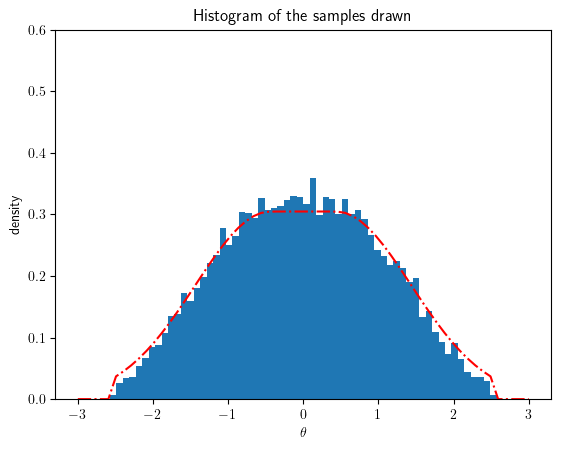
\includegraphics[width=0.48\textwidth]{./Thesis/images/chapter3/example_marginal.png}
      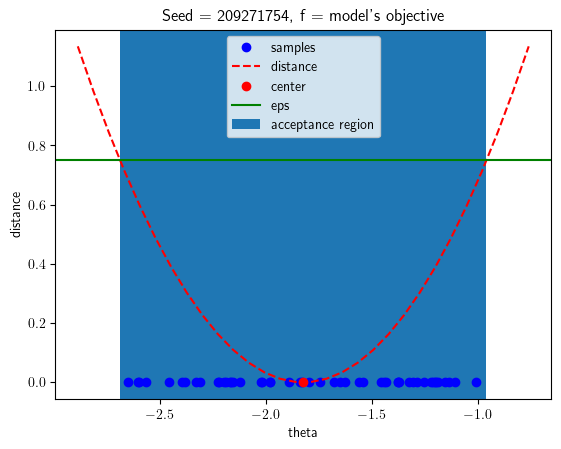
\includegraphics[width=0.48\textwidth]{./Thesis/images/chapter3/example_region_samples.png}
    \end{center}
  \caption[Histogram of the obtained samples at the 1D example.]{(a) Left: Histogram of the obtained samples. (b) Right: Acceptance region around $\theta_1^*$ with the obtained samples plotted inside.}
  \label{fig:example_sampling}
\end{figure}

\subsubsection*{Example - Evaluate Posterior}

The \pinline{romc.eval_unnorm_posterior(theta)} evaluates the
posterior at point $\theta$ using expression
\eqref{eq:aprox_posterior}. The \pinline{romc.eval_posterior(theta)}
approximates the partition function
$Z = \int_{\thetab} p_{d,\epsilon}(\thetab|\data) d\thetab$ using the
Riemann approximation as explained above. In our simple example, this
utility can provide a nice plot of the approximate posterior as
illustrated in figure~\ref{fig:approx_posterior}. We observe that the
approximation is quite close to the ground-truth posterior.

\begin{figure}[ht]
    \begin{center}
      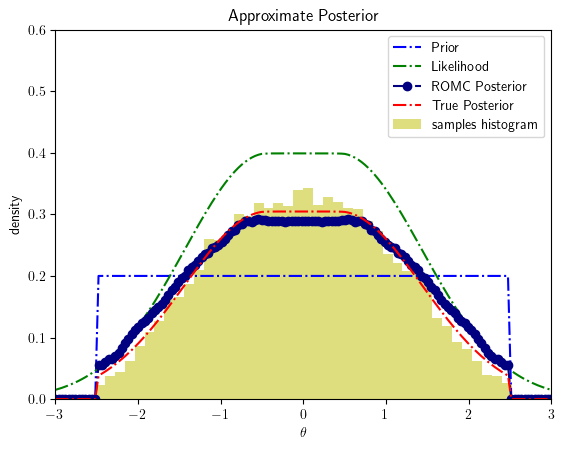
\includegraphics[width=0.75\textwidth]{./Thesis/images/chapter3/example_posterior.png}
    \end{center}
  \caption[Approximate posterior evaluation, at the 1D example.]{Approximate posterior evaluation.}
  \label{fig:approx_posterior}
\end{figure}


\subsubsection{Evaluation part} 
\label{subsec:evaluation}
The ROMC implementation provides two functions for evaluating the inference results,

\begin{enumerate}[label=(\roman*)]
\item \mintinline{python}{romc.compute_divergence(gt_posterior, bounds=None, step=0.1,}

      \mintinline{python}{                        distance="Jensen-Shannon")}

\item \mintinline{python}{romc.compute_ess()}
\end{enumerate}

\subsubsection*{Function (i): Compute the divergence between ROMC approximation and a ground-truth posterior}

\pinline{romc.compute_divergence(gt_posterior, bounds=None, step=0.1,}

\pinline{                     distance="Jensen-Shannon")}
\vspace{5mm}

\noindent
This function computes the divergence between the ROMC approximation
and the ground truth posterior. Since the computation is performed
using the Riemann's approximation, this method can only work in low
dimensional parameter spaces; it is suggested to be used for up to the
three-dimensional parameter space. As mentioned in the beginning of
this chapter, in a real-case scenario it is not expected the
ground-truth posterior to be available. However, in cases where the
posterior can be approximated decently well with a numerical approach
(as in the current example) or with some other inference approach,
this function can provide a numerical measure of the agreement
between the two approximations. The argument \pinline{step} defines
the step used in the Riemann's approximation and the argument
\pinline{distance} can take either the \pinline{Jensen-Shannon} or the
\pinline{KL-divergence} value, for computing the appropriate distance.

\subsubsection*{Function (ii): Compute the effective sample size of the weighted samples}

\mintinline{python}{romc.compute_ess()}
\vspace{5mm}

\noindent
This function computes the Effective Sample Size (ESS) using the
following expression~\autocite{Sudman1967},

\begin{equation} \label{eq:ESS}
  ESS = \frac{(\sum_i w_i)^2}{\sum_i w_i^2}
\end{equation}

The ESS is a useful measure of the \textbf{actual} sample size, when
the samples are weighted. For example if in a population of $100$
samples one has a very large weight (e.g.\ $\approx 100$) whereas the
rest have small (i.e.\ $\approx 1$), the real sample size is close to
1; one sample dominates over the rest. Hence, the ESS provides a
measure of the equivalent uniformly weighted sample population.

\newpage


\begin{pythoncode}
res = romc.compute_divergence(wrapper, distance="Jensen-Shannon")                                 
print("Jensen-Shannon divergence: %.3f" % res)
# Jensen-Shannon divergence: 0.025

print("Nof Samples: %d, ESS: %.3f" % (len(romc.result.weights), romc.compute_ess()))
# Nof Samples: 19950, ESS: 16694.816
\end{pythoncode}
